%!TEX program = xelatex
\documentclass[a4paper]{ctexart}

\usepackage{listings} 
\usepackage{geometry}
\usepackage{booktabs}
\usepackage{graphicx}
\usepackage{tabularx}
\usepackage{multirow}
\usepackage{enumitem}
\usepackage{url}
\usepackage[bottom]{footmisc}

\renewcommand{\multirowsetup}{\centering}

\geometry{
    left=23mm,
    right=23mm,
    top=23mm,
    bottom=23mm,
}

\setlength{\parskip}{0.5em}

\title{CodeOcean 商业模式文档}
\author{
  曾少勋 171250603\\
  刘洪禹 171840773\\
  黄国钊 171250530\\
  夏雨笛 171250011\\
}
\date{\today}

\begin{document}

\maketitle

\begin{abstract}
  本项目为 CodeOcean 小组在 2020 年春季学期《需求与商业模式创新》课程中大作业设计的同名项目,此文档为其商业模式设计文档。
\end{abstract}

\tableofcontents

\newpage

\setlength{\parskip}{1em}

\section{度量数值}
文档中总共有4份客户洞察移情图,9个候选创意,36点商业画布要点,30种画布要点联系;引用了10篇新闻和调研报告;提供了4+1个故事;每个场景包含了6个要点。


\section{客户洞察}

我们通过现实生活的观察与新闻等渠道,筛选并分析了一些其需求可以联系在一起的群体。

\subsection{高校和企业}
\begin{itemize}
  \item \textbf{看}:在线问答平台和教学平台涌现,这些平台大大降低了学习的成本,使得网络线上教育成为趋势;为了跟上这种趋势,国内外已经有大量的大学公布大量的公开课,这些公开课可以非常容易的获取和学习,有的甚至可以配套作业以及考试;随着网络上的资源越来越为普及,教育和学习不再局限于线下,网络线上教育成为趋势;同时,这些网络上的课程大多自成体系,往往是从传统的计算机基础课程发展而来,课程一般内容较多,时间跨度较长,对于基础知识的讲解比较细致,发布课程往往需要完整的课程设计。
  \item \textbf{听}:随着越来越多的人从事计算机编程相关方向的开发,有更多的学员期待学到编程知识;对大部头的课程需求变少,这些课程往往是在大学中就可以学到,或者是已经有了大量的经典教材和学习资料;而对于一些新兴的领域,或者是对于经验依赖较强的领域,教学资料又相对较少,因此更多学员不满足于基础知识,对高端进阶知识的需求增加;同时,因为知识更新的周期变短,在这样一个知识爆炸的时代,需要快速的获取新知识,对小而精的课程的呼声越发高涨。
  \item \textbf{想}:在本职工作外有额外的收入渠道;自身有着丰富的开发或教学经验,希望能传授自己丰富的行业知识和经验;自身认识的人不多,缺乏渠道和平台,难以建立自己的教育平台;希望能有效利用工作之余的碎片化时间。
  \item \textbf{说和做}:调查各个现有的网课平台;根据同事的情况作出选择;和同事一起开设网课做兼职。
  \item \textbf{痛处}:因为已有本职工作,因此面临时间的碎片化问题;希望对自己本职工作的影响越小越好;开设的课程受众要广,可以复用自己的劳动成果。
  \item \textbf{收益}:额外的收入;灵活可调配的时间;帮助他人的成就感;学员的良好反馈;不需要自己投入大量精力。
\end{itemize}

\begin{center}
  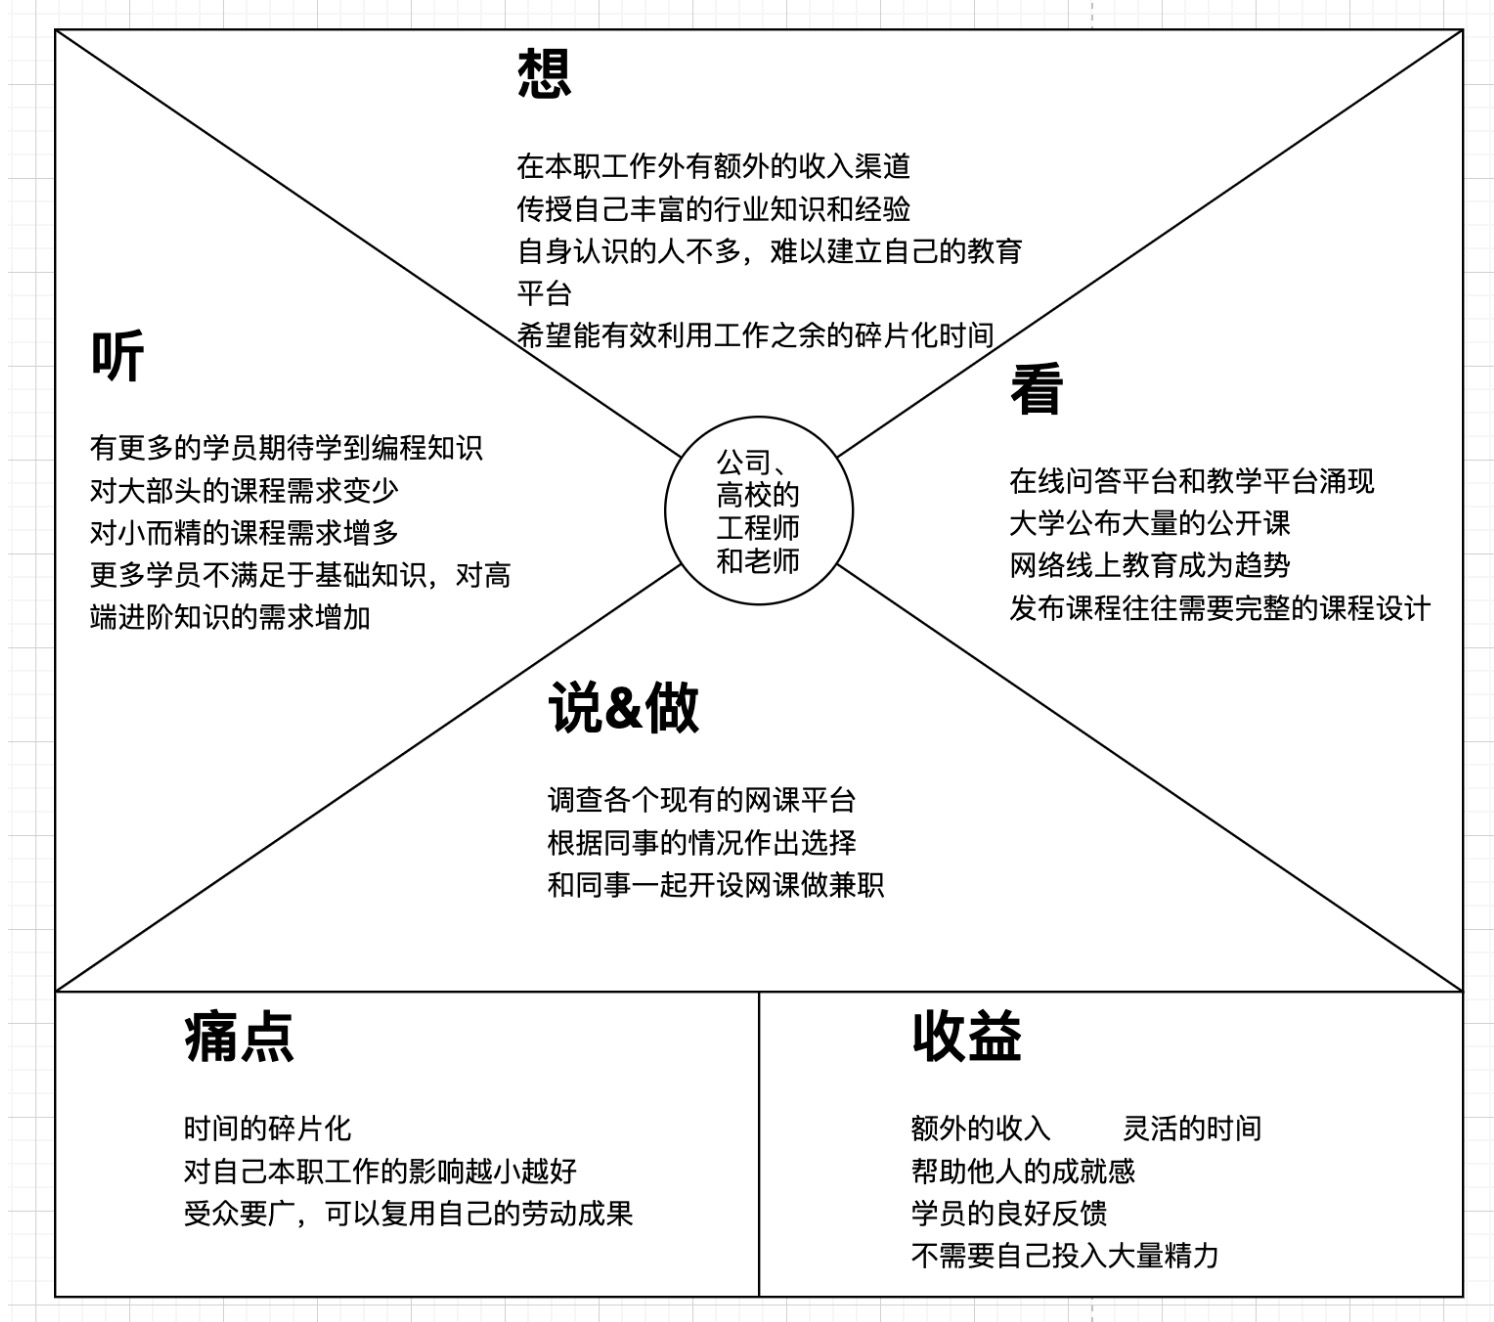
\includegraphics[width=14cm]{高校和企业.png}
\end{center}

\subsection{兼职大学生}
\begin{itemize}
  \item \textbf{看}:大学生到了需要自己计划开销的年纪,常常需要更多的开销,却不好意思向父母开口,很多人会选择通过兼职的方式获取外快。
  \item \textbf{听}:各种大学生兼职被骗的新闻层出不穷:有的大学生被克扣工资;有的大学生在毫不知情的情况下从事了违法行业;有的大学生被引诱着签署了不平等的协议,从而莫名其妙的背上了高额的“违约金”……
  \item \textbf{想}:希望能利用自己熟悉的技能赚取外快,在赚钱的同时也提升了自己。
  \item \textbf{说和做}:现在的大学生往往会通过学长、学姐的推荐,看网络上的口碑等方式来选择兼职平台。
  \item \textbf{痛点}:大学生即使自己拥有较高的编程能力,却往往会从事发传单、收银员、图书管理员等职位,难以在自己擅长的领域发挥实力。同时,由于自己是学生身份,要以学业为主,至少半天起算的兼职时间常常难以挤出。
  \item \textbf{收益}:大学生除了获得金钱,还希望能在兼职中锻炼自己的能力。
\end{itemize}

\begin{center}
  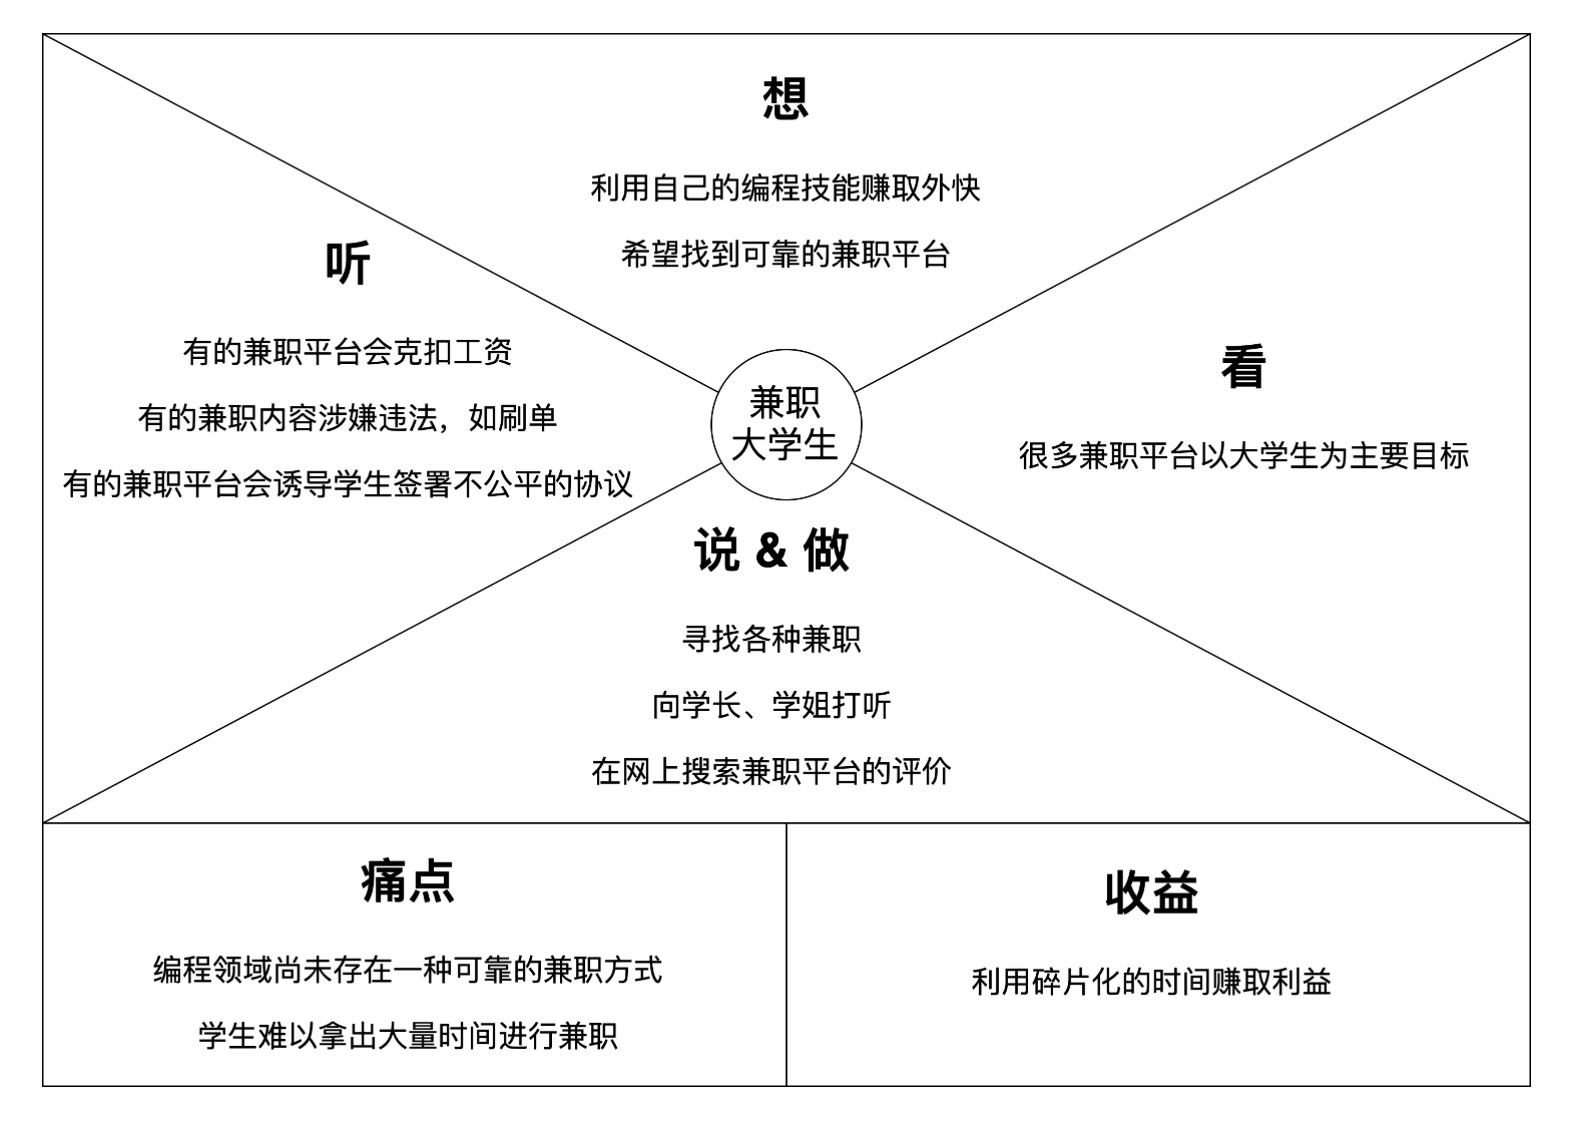
\includegraphics[width=14cm]{兼职大学生.png}
\end{center}

\subsection{提问者}
\begin{itemize}
  \item \textbf{看}:有的编程作业的环境复杂,提问者无法将自己的环境清楚描述给解答者;甚至他们不清楚自己的问题在哪里,找不到人一对一解答;虽然现有很多可以在线运行代码的提问平台,但沙箱都提供的是标准环境,不能体现提问者的本机环境,因此不能直接应用答者的修改到问题代码上。
  \item \textbf{听}:身边的朋友和他有一样的困扰;老师给他推荐了很多编程教学的网站,却都不是很满意。
  \item \textbf{想}:想拥有一个集“代码展示、在线IDE、配置环境的一致性描述、bug可复现、直观呈现修改前后对比”为一体的平台;想拥有一个随叫随到为自己解答问题的人。
  \item \textbf{说和做}:和身边的人吐槽:提问代码细节有关的问题会花费大量时间,需要很多交流成本;不断尝试各种编程教学平台。
  \item \textbf{痛点}:问答双方交流成本高——存在不能一次性定位并且解决bug的现象;很难找到愿意花时间为自己解决问题的人;看文档学习的时候很难和自己的代码联系起来。
  \item \textbf{收益}:问题描述简单方便,能得到有针对性的、有效的解答、一矢中的;随时有解答小哥来答疑解惑;利用代码沙盒帮助学习编程。
\end{itemize}

\begin{center}
  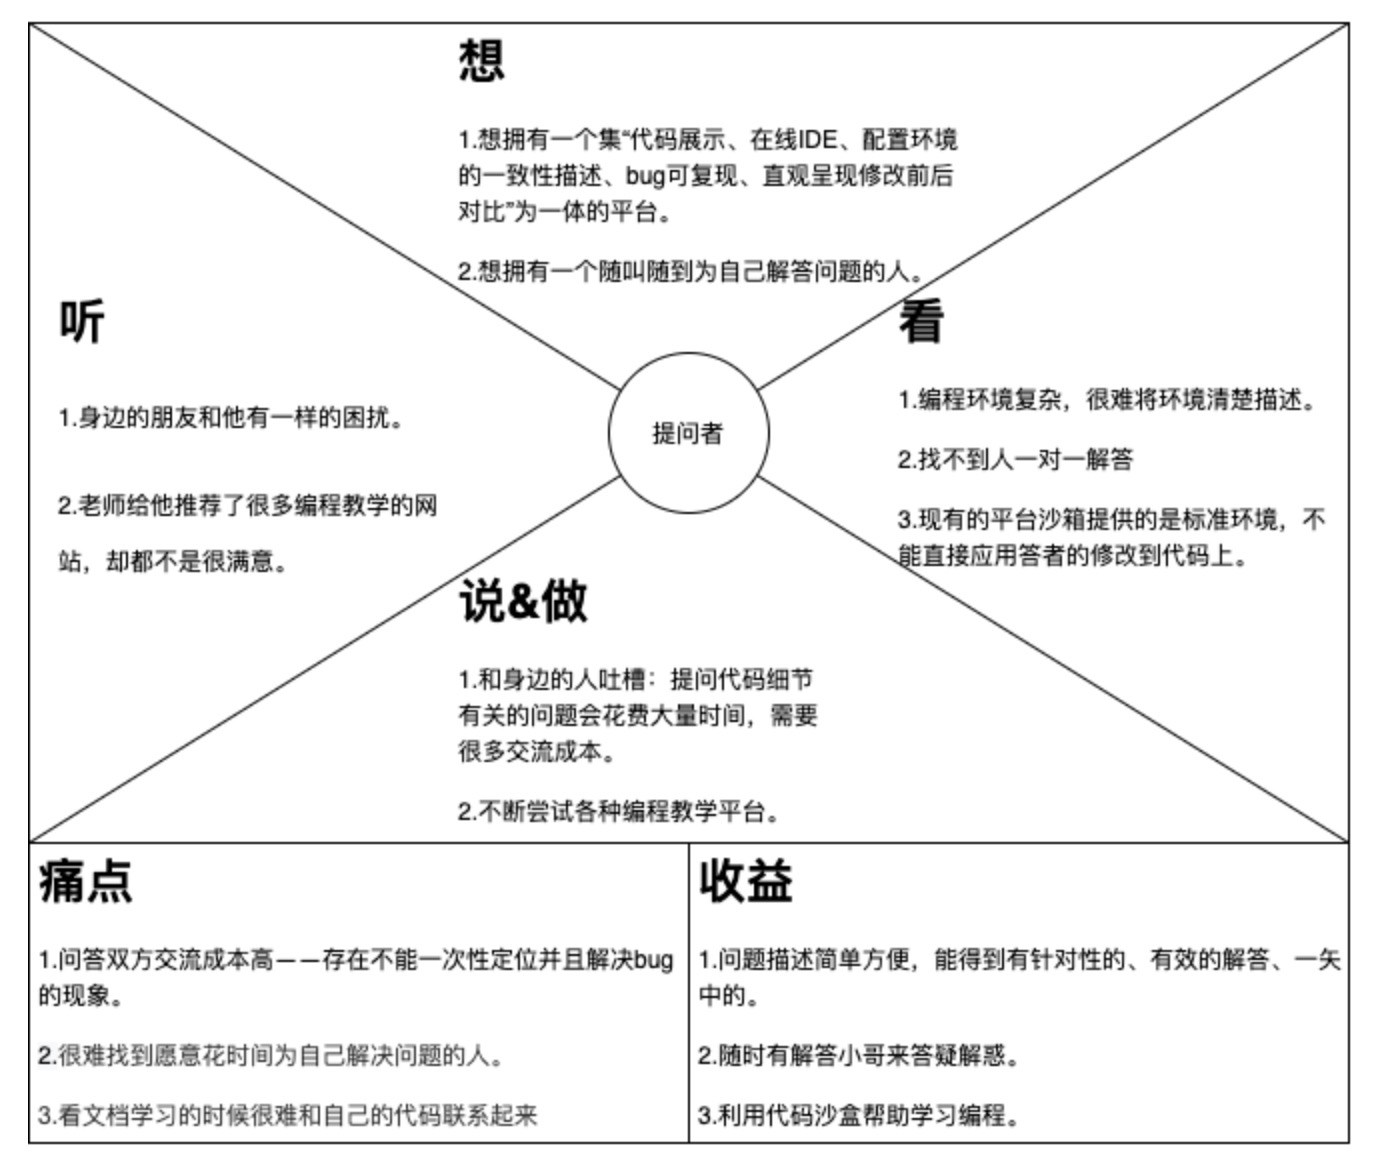
\includegraphics[width=14cm]{提问者.png}
\end{center}

\subsection{编程学员}
\begin{itemize}
  \item \textbf{看}:在线教育平台不断出现;在互联网上的学习与投身互联网行业形成良性闭环;通过互联网进行自学需要在资源整合上付出许多时间。
  \item \textbf{听}:互联网发展成为社会大趋势;IT行业工资高,存在一定的人才缺口;在线教育平台良莠不齐。
  \item \textbf{想}:希望找到合适的编程教学平台,资源丰富,企业化气息低,风格自由,不会对学员有太多限制。
  \item \textbf{说和做}:留迹于Mooc,可汗学院等富有高校气息的公共在线教学平台;也会尝试企业的教学平台。
  \item \textbf{痛点}:在线教学平台对课程的附加服务太多;课程质量不佳花了冤枉钱;一门课程的学习周期往往比较长,以致半途而废;学习过程缺乏实践以致往往不能牢固地记住知识。
  \item \textbf{收益}:在线教学平台资源丰富,能找到自己感兴趣的课程;课程质量高,性价比高,能让自己收获颇丰;课程紧跟互联网发展趋势,知识能跟上时代,有助自己深入IT行业;课程知识有应用空间,能让自己试手加深印象。
\end{itemize}

\begin{center}
  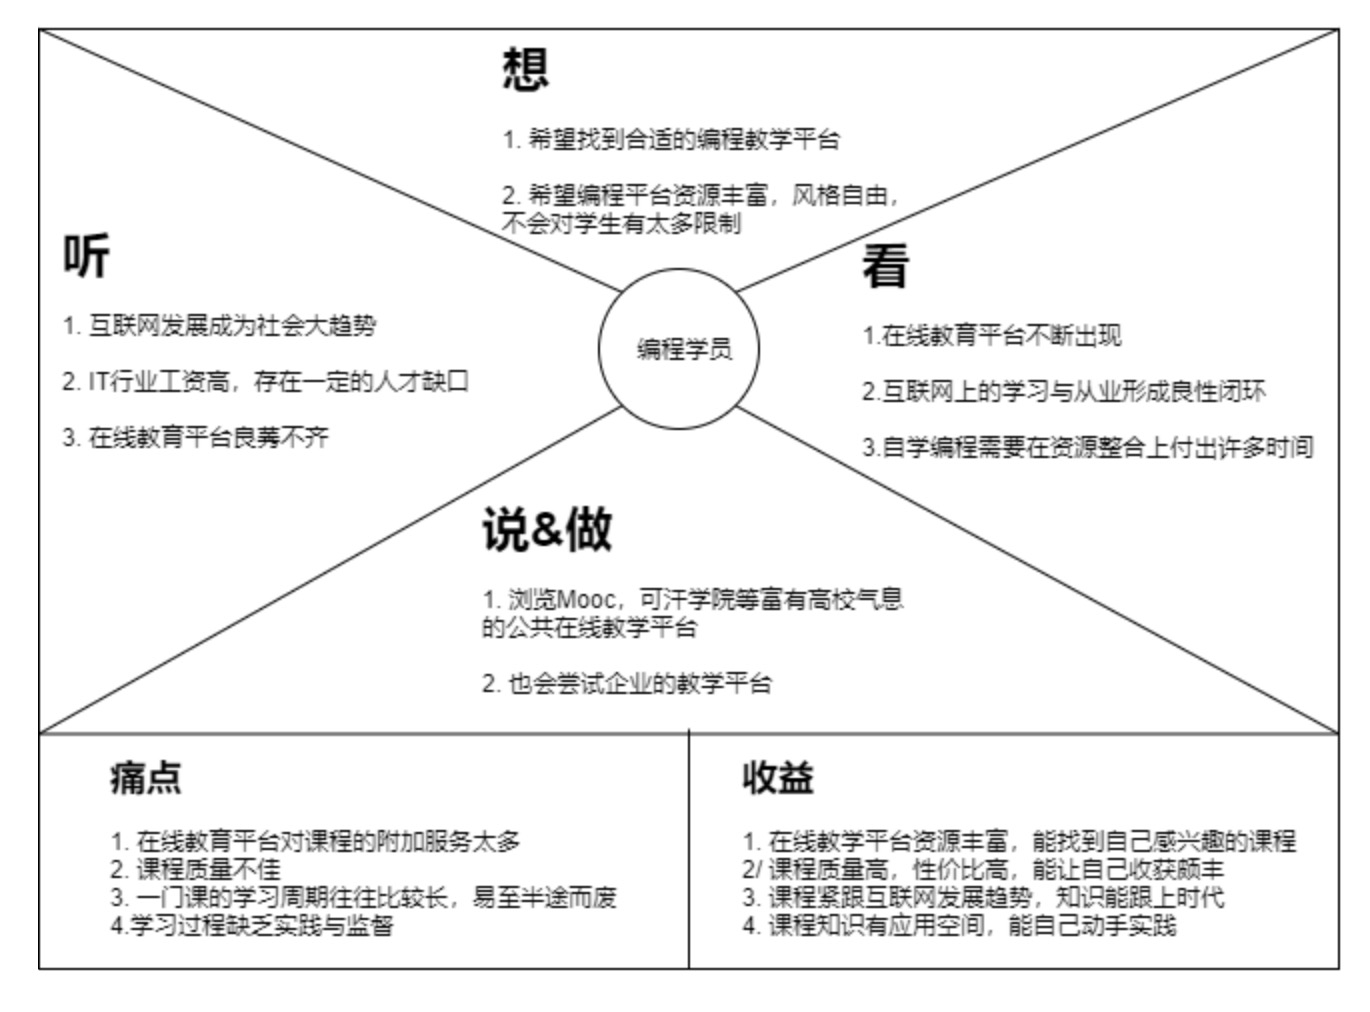
\includegraphics[width=14cm]{编程学员.png}
\end{center}

\section{构思}

\subsection{基本商业构思}
根据以上的客户洞察,我们认为可以使用一个平台来联系这些群体,通过平台的联系,可以满足其提问,教学或者赚外快的需求。CodeOcean平台基本上由问答社区、网课教学社区、项目文档社区组成,通过其功能及功能之间的相互联系来满足上述群体的需求。

\subsection{候选商业模式创意}
\subsubsection{创意一}
资源驱动:通过与高校和企业的合作,保证了平台优质的答题者以及工程师和老师。

如果平台已经拥有了一大批优秀的回答者和课程的提供者会怎么样?
\begin{itemize}
  \item 这会增加一部分的成本,因为维护这样的合作关系不仅需要平台提供人力来进行管理,而且可能还需要付出一定的费用,以持续吸引和维护这样的优质人群。
  \item 优质的回答者和网课资源也会吸引来大量的用户,这些用户在平台上提问问题会吸引来更多的人回答问题,形成良性循环;用户的增多也会让网课的播放量增多,这样也会吸引来更多的课程生产者。
  \item 提供的回答和开设的课程会形成平台的核心资源,这些知识性资源将塑造品牌形象,并且可以作为资源出售给其他平台。
\end{itemize}

对整个商业模式画布的影响:
\begin{itemize}
  \item 成本部分需要增加一部分的宣传成本和维护优秀的回答团队的成本。
  \item 因为问答用户的良性循环,会形成共同创造的社区氛围,这样在客户关系中很重要的部分就是社区和共同创。造
  \item 核心资源的知识性资源指的主要就是问答资源。
\end{itemize}

\subsubsection{创意二}
成本,技术驱动:通过云上的部署来缩减成本。

如果平台的代码沙盒功能是架构在云端的docker容器上会怎么样?
\begin{itemize}
  \item 因为有大量的问答,每个问答都需要docker环境来支撑,如果使用购买服务器的方式来扩充存储,那么将会造成服务器的资源压力大,而且可能会有大量的闲置资源,因为问题被解决之后对应的docker的使用频率就会大大降低,因此如果全部架构在云上,可以做到弹性扩容,而且对初期来说,只要付出极少的成本就可以快速搭建起服务。
  \item 进一步,随着业务的成熟和规模的扩大,我们可以维护自己的云开发团队,未来也有可能提供云服务,或是为其他网站提供代码沙盒的功能,使得其他网站也可以使用代码沙盒来展示和用户互动。
\end{itemize}

对整个商业模式画布的影响:
\begin{itemize}
  \item 成本降低,不需要维护大量的服务器,初期只需要购买云服务的资源即可。运维的成本也随之大大降低。
  \item 未来计划的关键业务可以增加一条:为其他平台提供一个云端的docker的代码运行环境,提供给其他企业或平台一个代码展示、运行和共享的容器环境,封装后台复杂的管理细节,提供简单的接口供其调用。
  \item 根据第二条,未来收入来源有可能增加:租赁给其他平台的docker资源、开发的收费api接口,以及后续的运行维护费用。
\end{itemize}

\subsubsection{创意三}
创新驱动:为用户提供一种新颖的、便捷的问答方式。

如果平台平台提供的问答方式足够便捷会怎样?
\begin{itemize}
  \item 便捷的提问方式会降低提问门槛,使得用户更愿意提问,增加潜在的用户数。
  \item 便捷的回答方式降低提问者与回答者之间的沟通成本,使得问题更容易、更快地得到解答,增加平台的优质回答数量,从而吸引更多的用户。
  \item 提供大量的代码沙箱需要大量的云计算资源,会增加一定的服务器成本。
\end{itemize}

对整个商业模式画布的影响:
\begin{itemize}
  \item 一定程度上增加了成本。
  \item 加快社区规模与发展速度,强化客户关系。
  \item 会让用户创造更多的核心资源。
\end{itemize}

\subsubsection{创意四}
广告驱动:广告是平台收入的一大部分。

如果增加广告数量会怎样?
\begin{itemize}
  \item 平台与更多的广告商进行合作,获取的广告费用会增加,广告转化率也越高。
  \item 过多的广告会影响用户体验,造成一定程度的客户流失。
  \item 大量的广告会“喧宾夺主”,干扰用户的学习过程,影响学习效果,与“沉浸式”学习的发展趋势不符。
\end{itemize}

对整个商业模式画布的影响:
\begin{itemize}
  \item 强化了与广告商的合作。
  \item 作为平台核心资源的用户数量会因此下降。
  \item 一定程度上违背了价值主张。
\end{itemize}

\subsubsection{创意五}
客户驱动:根据客户需求和特点确定平台业务展开方向。
资源驱动:根据平台可以利用的资源范围创造业务,保证业务是可行的。

如果平台要提供各种各样大量的网课教学视频会怎么样?
\begin{itemize}
  \item 需要增加一部分人力成本。需要人为审核网课资源质量,给不同难度的网课进行分类。这样可以使用户在选择网课的时候能很快选到自己需要的。
  \item 吸引更多的用户。丰富的网课教学视频涵盖的领域非常广泛,使一些小众的用户也可以在平台上找到自己需要的网课视频。(长尾商业模式)
  \item 需要增加更多高校企业教师的合作费,增加成本的压力。
\end{itemize}

对整个商业模式画布的影响:
\begin{itemize}
  \item 需要增加一部分审核分类网课的人力成本,增加更多的高校企业教师的合作成本。
  \item 可以划分各种不同技术栈的用户,无论是使用大众的语言的用户,或者是使用小众语言的用户,都可以找到相应的网课教学。
\end{itemize}

\subsubsection{创意六}
成本驱动,技术驱动:考虑资源过多对成本的影响并且技术上降低成本的可能性。

如果平台已经有了很多知识性资源会怎么样?
\begin{itemize}
  \item 实物资源和人力资源的投入也要增加,更多的知识性资源需要更多的服务器来支撑,同时也需要更多的开发维护人员来保证多并发的安全性和响应资源的速度。
  \item 知识性资源的丰富可以将一部分知识性资源免费提供给用户,另一部分资源进行收费。这样在吸引用户的同时也保证了平台的收入来源。(免费商业模式)
  \item 可能有的资源太过于小众,点击率太低。但仍然要支付合作费用造成浪费。
\end{itemize}

对整个商业模式画布的影响:
\begin{itemize}
  \item 知识性资源增加的同时实物资源和人力资源的投入也要增加。
  \item 增加课程费,解答费带来的收入来源。
  \item 由于资源过于小众,增加不必要的成本。
\end{itemize}

\subsubsection{创意七}
客户驱动,财务驱动:用成本较低的办法吸引吸引足够多的用户,以创造更多的收入。

如果平台的问答社区氛围不足会怎么样?
\begin{itemize}
  \item 先把重心放在课程社区建设与文档社区建设,吸引足够多的使用用户后,再通过优惠等激励措施引导用户参与进问答社区的建设。
  \item 加大宣传,请有名的编程界人物或者捏造用户故事作为宣传,或者与相似平台合作获得引流来建设问答社区。
\end{itemize}

对整个商业模式画布的影响:
\begin{itemize}
  \item 平台在前期的结构不完全,问答板块可能尚未成长为"社区"
  \item 平台发展过程中的成本结构与收入来源的各成分比重会随时间变化,前期需要花费一些额外费用(宣传等)来帮助建立社区氛围,社区足够大后,相关的收入(问答费用抽成)才足够显著。
  \item 平台的社区价值主张在前期主要依靠平台自身进行宣传和推广,有足够大的用户群体后才能自发地维护和建设社区氛围。
\end{itemize}

\subsubsection{创意八}
资源驱动:拓展可用的合作资源。

如果有IT行业的经验工作者希望以个人作为课程开设者寻求合作关系会怎么样?
\begin{itemize}
  \item 建立合作关系,和与企业和高校的合作关系类似,允许其在平台上担任教师来授课,同时平台抽取一定的课程费用作为收入,除此之外也可以让其以主动的姿态参与进问答社区的建设中,他在促进平台发展的同时也间接提升能接触到自身开设的课程的人数,双方都能受益。
  \item 在与其合作一段时间后,平台可以通过其作为沟通桥梁,与其就职的企业联系,探索合作的可能。
  \item 
\end{itemize}

对整个商业模式画布的影响:
\begin{itemize}
  \item 客户细分获得拓展,作为个体的IT工作者也是一种潜在用户群体。
  \item 合作关系获得拓展,个体工作者也可以作为合作对象,与企业可能存在由个体工作者连接起的联系。
\end{itemize}

\subsubsection{创意九}
资源驱动,财务驱动:更紧密的合作关系增加了可用的资源,利用资源以来增加收入,降低成本。

如果与某家企业建立了紧密合作关系会怎么样?
\begin{itemize}
  \item 平台的宣传对于与该企业密切相关的实体的可达性大大增强。
  \item 企业的员工可以参与到社区中,可以作为积极的回答者,或者公司自开发工具的文档及示例代码的,员工整体作为一家企业的形象可以使企业居于更高的宣传地位。
\end{itemize}

对整个商业模式画布的影响:
\begin{itemize}
  \item 重要合作中的与企业合作可以细分为多种形式(普通合作:旗下有一些员工作为课程教师与平台合作;紧密合作:员工参与进平台的课程,问答社区,文档区等多方面的建设;平台为企业提供更高的宣传地位)。
  \item 核心资源中的企业合作关系资源增加。
  \item 宣传企业的广告收益(合作的收入,包括直接的分成和潜在的帮助平台建设等作用)会增多。
\end{itemize}

\subsection{最终确定的商业模式创意}
\begin{itemize}
  \item \textbf{创意二}\ 使用云端docker作为代码沙盒,用于分发,讨论和修改,以带来环境的一致性,透明性和修改便利性,减少在细枝末节上的不必要的讨论。云服务器拥有可伸缩性,并且可以加上平台自身的docker服务后再出租。
  \item\textbf{创意五}\ 平台向拥有丰富的课程资源方向发展,在广度上,让对不同方向感兴趣的客户都能找到相关课程,时长上,推出时长长短不同的课程视频以应对不同的客户背景。
  \item\textbf{创意七与八}\ 拓展个体开发者成为重要合作关系之一,在开设课程、参与问答社区建设、和项目文档与代码的发布和维护上都可以探讨合作。
\end{itemize}

\section{视觉化思考}

\subsection{可视化画布}
\begin{center}
  \includegraphics[width=12cm]{可视化画布.png}
\end{center}

\subsection{相关分析}

根据详细讨论后,我们创造了一份可视化的商业模式画布,建立了CodeOcean平台的大致商业框架。

我们的主要目标客户一方面有对于编程有疑惑的学习者,可能遇到了难解的问题或者希望提升学习效率;另一方面有希望将自己的编程知识转化为便利的赚外快渠道的学生等。同时平台会寻求与企业/高校、个体开发者和相似社区的合作,共同建设课程社区、问答社区和项目社区等,以开展编程课程教学,有偿/无偿代码问题问答和项目demo沙盒化等业务,这些都会与docekr作为代码沙盒密切相关,因此docker沙盒本身也可以作为一项可出租资源,成为平台业务之一。围绕docker沙盒展开的业务也导出了创新与便捷价值主张,作为联系各方的平台,鼓励客户共同创造资源,建设社区也是平台的核心思想之一。我们更倾向建造一个自由而非个人商业气息很强的社区,类似stackoverflow。平台的重要资源不仅有常规的工作人员等人力资源和物理设施和服务器等实物资源,还有共同创造的知识资源,比如课程知识,问答平台的高质量答案,以及项目文档与demo等。平台通过自身的渠道(广告等)与合作方的宣传渠道来推广该平台。

\section{模型构建}

经过对商业画布的精细化和补充,我们最终建立了一个商业模型。

\subsection{商业模式画布}

\begin{center}
  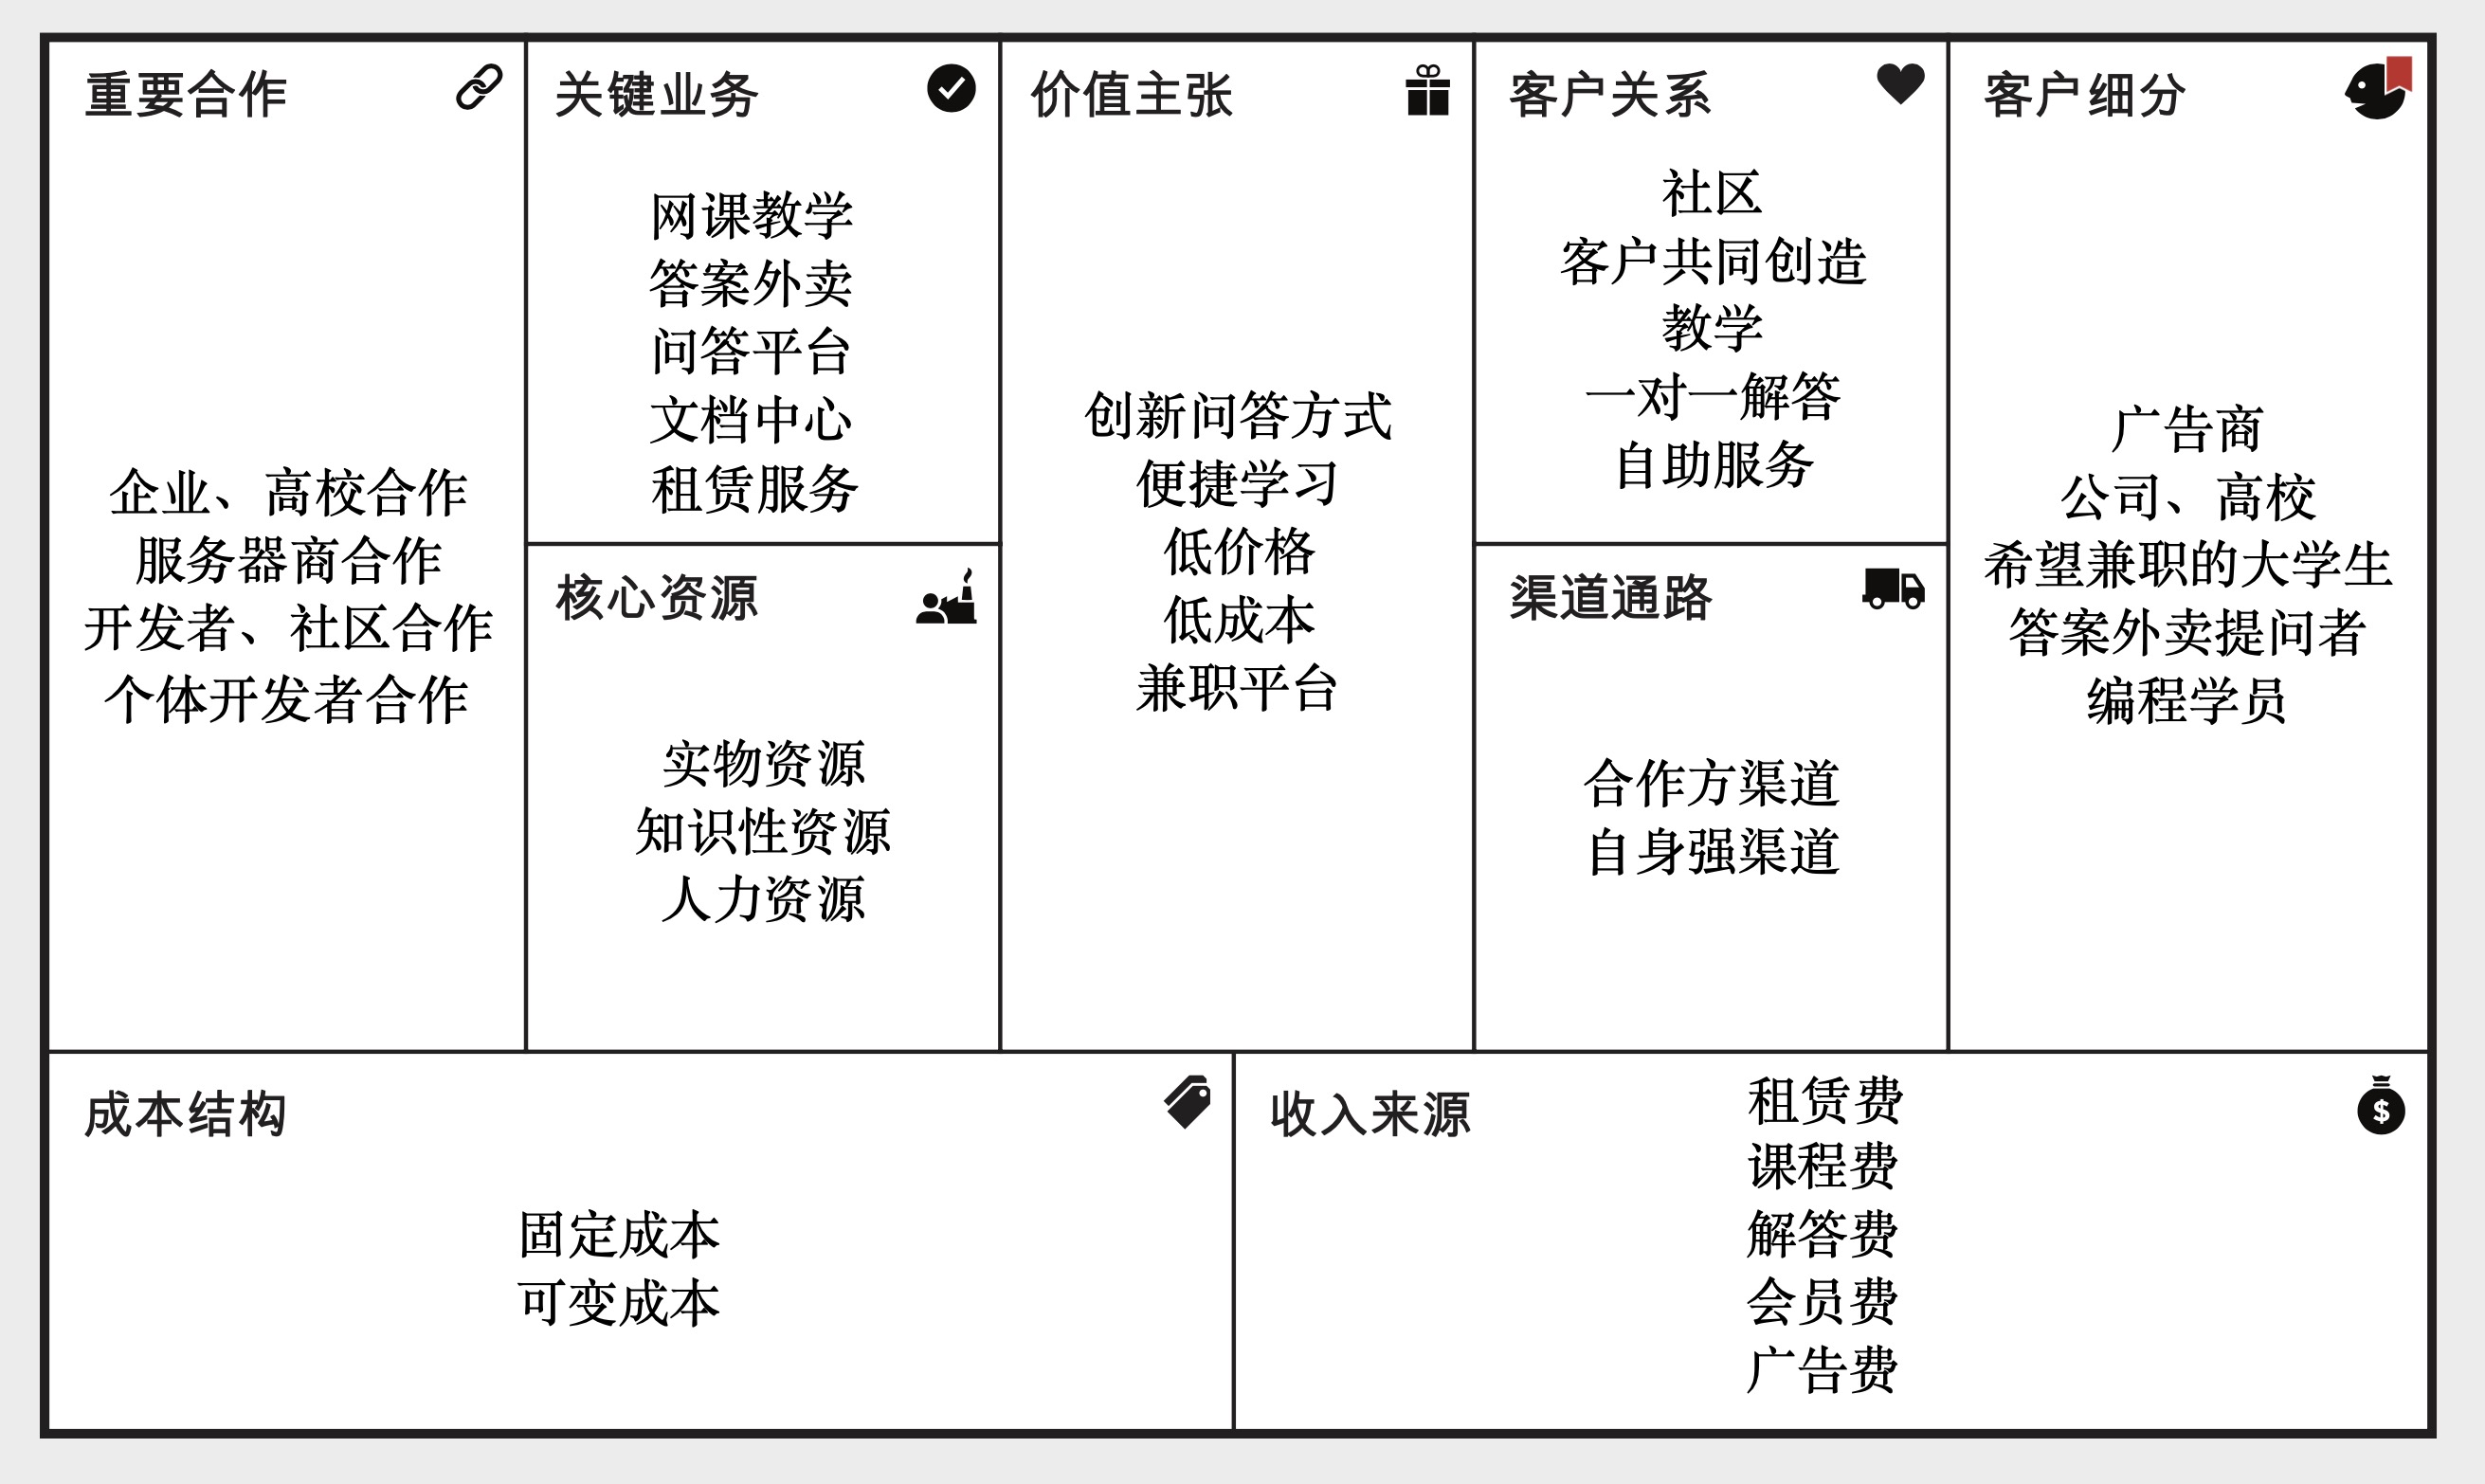
\includegraphics[width=13cm]{canvas.png}
\end{center}

\subsection{商业画布要点}

\subsubsection{关键业务}

\begin{enumerate}[label=\alph*.]
  \item 网课教学:提供优质课程,通过录播、直播、作业(OJ)、考试等方式,帮助用户学习掌握新知识。课程有长期和短期两种,详见项目简介中的对应模块介绍。
  \item 答案外卖:提问者可以提出问题,支付一定的解答费,会有“解答小哥”接单并提供一对一解答。在问题解决后,提问者与“解答小哥”会进行双向评价,基于好评制度保证解答的质量。“解答小哥”会获得一定比例的解答费作为报酬,好评率高的还可以获得额外奖励。详见项目简介中的对应模块介绍。
  \item 问答平台:基于 docker 与在线版 vscode,提问者提问时,平台会自动生成 docker 环境,并在启用运行在线版 vscode,提问者将问题代码复制到此环境中复现问题,解答者打开网页即可修改并实时看到结果。解答者提交解答后,其修改内容会自动以 diff 的形式展现,使得后来者可以一目了然。详见项目简介中的对应模块介绍。
  \item 文档中心:收集了各大项目官方文档,同时允许用户贡献,基于 wiki,使得所有人都可以自由编辑,文档中的代码可以在直接沙盒中运行,用户可以随时修改并观察结果。详见项目简介中的对应模块介绍。
  \item 租赁服务:为其他平台提供一个云端的docker的代码运行环境,提供给其他企业或平台一个代码展示、运行和共享的容器环境,封装后台复杂的管理细节,提供简单的接口供其调用
\end{enumerate}

\subsubsection{价值主张}

\begin{enumerate}[label=\alph*.]
  \item 创新问答方式:现有的问答平台,在用户提出问题后,往往需要经过较长时间的等待才能获得答案。本平台提供的答案外卖服务,尚未在市场出现,用户可以通过支付一定的费用,让获取答案像叫外卖、打车一样简单,是一次创新的尝试。
  \item 便捷学习:用户在问答中心提问时可以直接将代码放入 docker,回答者可以直接在网页版 vscode 中回答,无需配置环境。文档中心中的代码都可以直接在沙盒中执行,便于用户修改、查看结果,提升了学习效率。
  \item 低价格:增加宣传力度,增加用户数量,降低课程价格,以量取胜。
  \item 低成本:答案外卖使得用户花费少量金钱即可解决问题,节约了用户大量的时间,使得用户可以做更多有价值的事情。
  \item 兼职平台:用户达到一定资质便可注册为“解答小哥”,接取答案外卖订单,并获得一定报酬,为大学生等群体创造了一个可靠的兼职平台。
\end{enumerate}

\subsubsection{客户关系}

\begin{enumerate}[label=\alph*.]
  \item 社区:对某一问题感兴趣的用户群可以就这一问题进行讨论,发表自己独到的见解和解题思路,从而形成社区。
  \item 客户共同创造:任何用户都可以在问答平台上提问或解答,同时任何用户也可以贡献出自己对于一些经典算法解答的代码沙盒。人人都可以在平台上创造资源和使用资源,使平台的资源更加丰富。
  \item 教学:平台老师可以开设线上课程教学,其他对这一课程感兴趣的用户可以来听课。
  \item 一对一解答:用户可以通过答案外卖获得专属私人服务,一对一讲解为用户提供私人咨询。
  \item 自助服务:用户可以借助代码沙盒进行练习,自行搜索相关解答、提出问题,浏览文档。
\end{enumerate}

\subsubsection{重要合作}

\begin{enumerate}[label=\alph*.]
  \item 企业、高校合作:教学课程是平台关键业务的重要一环。与企业、高校合作,既能通过规模效应减少联系资深人士在平台上开设课程的平均成本,也能有效延长讲师在平台驻扎的年限。
  \item 服务器商合作:与服务器商合作,为其提供宣传,推荐用户在学习中使用,可以为其增加潜在用户,同时本平台也能优惠使用其服务。
  \item 开发者、社区合作:与各软件项目的开发者、开发社区合作,平台整理和收录其开发的项目的文档,开发者和社区可以通过 docker 部署一些简单的项目使用代码,帮助新手更快地上手其开发的工具,对于平台和项目的宣传都有促进作用,实现双赢。
  \item 个体开发者合作:与个体开发者合作,开设课程
\end{enumerate}

\subsubsection{收入来源}

\begin{enumerate}[label=\alph*.]
  \item 课程费:教师可以开设一些付费课程,可以是长期的大型课程,也可以是一些短视频小课,用户需要付费才能查看这些课程的内容,该网站为这些课程提供平台,相应地收取一些课程收入的抽成作为回报。
  \item 解答费:用户解答费用的抽成。用户可以通过付费可以对认证用户进行私下的问题咨询,类似地网站会抽取一定比例的费用作为提供平台的回报。
  \item 会员费:因为存在短期课程,网站开设会员制度,会员可以免除学习短期课程的费用,与教师的分成可以具体讨论。
  \item 广告费:网站提供一些区域作为发布广告的场所,从广告厂商处收取费用。
  \item 租赁费:租赁给其他平台的docker资源、开发的收费api接口,以及后续的运行维护费用。
\end{enumerate}

\subsubsection{核心资源}

\begin{enumerate}[label=\alph*.]
  \item 实物资源:所拥有的实物资源主要是为了支持系统的在线平台,因此需要高性能的服务器,以满足大量用户的代码沙盒的使用需求。
  \item 知识性资源:主要由用户生产的资料组成。包括开设的课程、用户提出的问题以及回答、用户发布的文档,这些共同组成了平台的知识性资源。
  \item 人力资源:包括开发人员和核心的用户。平台的开发团队、招募或认证的师资队伍、解答问题的工程师队伍、出色的回答者都是重要的人力资源。
\end{enumerate}

\subsubsection{成本结构}

\begin{enumerate}[label=\alph*.]
  \item 固定成本:包括雇用开发人员的成本、维护物理服务器的成本、管理员工工资、机房用电、网络费用等。这些支出不论平台是否正常运行都需要支付,因此归为固定成本。
  \item 可变成本:包括雇用维护人员的成本、雇用客服人员的成本,此外,该系统需要有服务的提供者(课程的开设和问题的回答者),因此为了让平台有一些初始化的课程内容和认证工程师,还需要支付聘请公司、高校教师的合作费、平台的宣传推广费。这些支出是平台运行时决定的,因此归为可变成本。
\end{enumerate}

\subsubsection{渠道通路}

\begin{enumerate}[label=\alph*.]
  \item 合作方渠道:与企业、高校的合作与宣传,与已有项目的合作与宣传,可以迅速提升知名度。同时,高品质的企业、高校可以提供优质的课程,从而吸引用户付费学习,与此同时,企业、高校举办的直播、答疑等交流活动也可以进一步提升评价。
  \item 自身强渠道:平台吸引部分想获得额外收益的高水平人群,作为“解答小哥”一对一回答问题,通过评价制度保证服务质量,从而获得良好的口碑,进一步提升知名度。
\end{enumerate}

\subsubsection{客户细分}

\begin{enumerate}[label=\alph*.]
  \item 广告商:投放广告,增加流量。
  \item 公司、高校:开设课程,赚取课程费。
  \item 希望兼职的大学生:成为“解答小哥”,通过解答问题获取收益。
  \item 答案外卖提问者:通过答案外卖服务,支付解答费,获得一对一解答。
  \item 编程学员:参加课程、浏览文档、问答社区。
\end{enumerate}

\subsection{商业画布要点联系}

\paragraph{1a(网课教学), 4a(企业、高校合作)}由于要开设网课程,因此需要和高校或是企业合作,以此来获得优质的师资开设网上课程。
\paragraph{1a(网课教学), 5a(课程费)}平台提供付费课程,当用户购买课程后,平台可以从用户支付的课程费中抽取一定比例,作为平台收入的一部分。
\paragraph{1b(答案外卖), 2b(兼职平台)}“解答小哥”可以通过解答问题获取收益,使得本平台成为一个可靠的兼职平台。
\paragraph{1b(答案外卖), 5b(解答费)}在用户使用答案外卖服务的同时,平台会抽取解答费的一部分作为收入。
\paragraph{1b(答案外卖), 7b(可变成本)}客服对于有争议的问答交易进行审查也是不确定的成本。
\paragraph{1c(问答平台), 2a(便捷学习)}基于 docker 的服务体现了便利性,用户之间的交流成本更低。
\paragraph{1d(文档中心), 4b(开发者、社区合作)}为了提供优质的文档,需要和大量的项目作者、社区进行合作。
\paragraph{1e(docker资源出租), 5e(租赁费)}新增业务提供docker的租赁服务,因此收入来源也相对应的增加了一条。
\paragraph{2a(创新问答方式), 3d(一对一解答)}通过平台为用户提供了创新问答方式这一价值主张,提问者随时提问,业内高手一对一解答,创建了一个便捷提问的平台。
\paragraph{2b(兼职平台), 4a(企业、高校合作)}平台为一些高水平用户提供了额外的收入渠道,使得企业、高校更加愿意合作。
\paragraph{3b(客户共同创造), 6b(知识性资源)}本平台只是提供了一个用户自由问答、编写文档的地方,用户所实际受益的资源,大部分都来自其他用户的贡献,而这正是本平台的核心资源之一。
\paragraph{3c(教学), 4a(企业、高校合作)}希望接受相关知识教育的人群是潜在客户,与企业、高校的合作能在宣传和教育资源上帮助吸引目标群体。
\paragraph{4a(企业、高校合作), 6b(知识性资源)}与企业、高校的合作可以为本平台提供十分优质的课程资源,这是本平台的核心资源之一。
\paragraph{4a(企业、高校合作), 7a(可变成本)}与服务器厂商的合作能降低服务器成本。
\paragraph{4b(企业、高校合作), 7b(固定成本)}与企业、高校的长期合作能降低联系成本。
\paragraph{6a(实物资源), 7a(固定成本)}核心资源中的服务器等资产属于必须要支付的固定成本。
\paragraph{6c(人力资源), 7b(可变成本)}招募师资队伍、工程师队伍需要根据各人水平不同支付不同的薪水,平台的前期建设有时需要根据情况聘请一些知名开发者帮助建设,都属于可变成本。
\paragraph{7b(审核人员工资), 6c(人力资源)}增加了平台审核分类网课的人之后,平台获得了更多人力资源,相应也要支付他们一些工资,这也同时增加了成本。
\paragraph{2b(兼职平台), 5a(课程费), 5b(解答费)}平台主张提供便捷提问渠道的同时,抽成用户的解答费用产生收入。
\paragraph{4a(企业、高校合作), 5a(课程费), 5c(会员费)}与企业、高校形成合作关系能增加开设课程的数量,用户会有更多的课程可以选择,平台在课程上的收入会增加,也能吸收更多的会员,增加会员费收入。
\paragraph{4c(开发者、社区合作), 5b(解答费), 5d(广告费)}与项目开发者、社区合作,吸引用户,促进社区建设增加,促进使用答案外卖的人群数量增加,广告收益增加。
\paragraph{8a(合作方渠道), 9a(广告商), 9b(公司、高校)}众多的合作方渠道使得有许多利益相关方均可通过本平台获益,使得本平台客户多边化,受众广泛、来源稳定。
\paragraph{2a(便捷学习), 2b(兼职平台), 9a(广告商), 9b(公司、高校)}平台主张提供用户咨询服务或者额外收入,可以满足不同类型人员的需求,是多边平台的表现。
\paragraph{3a(社区), 3b(客户共同创造), 3e(自助服务), 5b(解答费)}客户共同建设社区,形成良好氛围,鼓励提问,增加使用答案外卖的人群数量。
\paragraph{3a(社区), 3b(客户共同创造), 3d(一对一解答), 8b(自身强渠道)}平台所积累的优秀问题回答者,解答小哥,文档编写者成为了平台的自身强渠道,他们的服务为本平台创造了良好的口碑,同时,众多优秀人员的推荐也是本平台的良好宣传。
\paragraph{4a(企业、高校合作), 4b(服务器商合作), 4c(开发者、社区合作), 8a(合作方渠道)}与企业、高校、服务器商、开发者、社区的合作,在为其带去收益的同时,也使得本平台收获了优秀的资源、良好的口碑,拓广了本平台的合作方渠道。
\paragraph{1a(网课教学), 1c(问答平台), 1d(文档中心), 6a(实物资源), 6b(知识性资源)}网络课程、问答帖子和文档等都属于知识性资源。同时,为了支撑这些平台功能的运营,需要大量的服务器,这属于实物资源。
\paragraph{3a(社区), 3b(客户共同创造), 3d(一对一解答), 3e(自助服务), 4b(服务器商合作)}平台收录其项目的文档,开发者使用 docker 搭载简单的项目 demo 参与社区建设,吸引更多用户,对双方都起到宣传作用。
\paragraph{5(收入来源), 8(渠道通路), 9(客户细分)}通过合作方渠道,与企业和高校的合作,可以吸引来高校的老师,或是企业的工程师,这是多边平台的服务提供方;同时也会吸引来学生,这些是多边平台中的服务的消费方。这些客户互动产生的费用,例如付费课程和解答费用构成了网站的收入来源。
\paragraph{4(重要合作), 6(核心资源), 7(成本结构)}教学和问答平台的业务需要大量的服务器,因而其是一项重要的核心资源,并且建立的社区也是需要建设的知识性资源之一。出于削减成本的要求,与适合的实体比如服务器厂商,企业、高校的资深人士和项目开发者的合作,可以有效削减成本。

\subsection{新闻、调研及相关分析}

建立商业模式模型后,我们查询了一些相关资料用于可行性的验证和进一步的修改。

\subsubsection{付费5000元换来四字答复 你愿意花钱提问大V吗?}
\begin{itemize}
  \item \textbf{画布元素}:客户、重要合作:平台的优秀回答者。
  \item \textbf{链接}:\url{http://www.xinhuanet.com/newmedia/2017-04/07/c_136189658.htm}
  \item \textbf{主要内容}:现今各种自媒体平台涌现出一大批所谓的大V,而有一些大V提供了费用高昂的一对一问答服务,往往一个回答需要用户付出的价格极高,但是仍有许多人趋之若鹜。
  \item \textbf{分析}:  这个新闻中的回答的问题虽然不是技术问题,有一定的噱头,但是也可以看出当代人对于这种“明星效应”的追捧。如果平台有了一大批优秀的回答者,其中不乏有行业内知名的专家学者,那势必能引来更多的用户。
  另外,除了所谓的“明星效应”,文中也讨论了付费问答在当今社会的可行性。可以看到,当前社会中越来越多的人愿意为知识付费,而且愿意为一对一的问答知识付费,因此可以看出,若是平台能拥有一大批优秀的回答者,一定会吸引来大量的客户,进而展开后续的社区互动等。
\end{itemize}

\subsubsection{为什么Docker适合初创公司?}
\begin{itemize}
  \item \textbf{画布元素}:成本:使用docker削减成本。
  \item \textbf{链接}:\url{http://www.guodongkeji.com/newsshow-24-2446-1.html}
  \item \textbf{主要内容}:这片报道主要分析了目前的IT初创公司的docker实践,以及这些实践给初创公司带来的正面影响。
  \item \textbf{分析}:  通过分析公司规模和docker使用程度,我们可以发现随着公司规模的扩大,docker的使用占比越来越多,这时因为docker有诸多的优点,例如可移植性、编制、快速部署等。这些优点大大加速了开发的效率,而且减少了运维和基础设施的成本。在docker的加持下,云计算更加普及、更加方便。而对于初创公司来说,使用docker不仅可以加速开发迭代周期,更可以弥补前期资本不足的劣势。
\end{itemize}

\subsubsection{女程序员兼职在线教育编程培训,副业工资超过主业工资}
\begin{itemize}
  \item \textbf{画布元素}:客户,重要合作:和公司合作开设网课和招募回答者。
  \item \textbf{链接}:\url{https://new.qq.com/omn/20191122/20191122A0PP4Q00.html}
  \item \textbf{主要内容}:程序员兼职开培训班,收入可观。现在越来越多的程序员开始开设各种编程教学班级,这项副业越来越成为一种趋势。
  \item \textbf{分析}:  我们平台预想的一个重要合作就是和企业中的工程师合作,邀请他们来开设线上课程。结合这则新闻可以看出,目前的程序员理想副业之一就是网课教学。但是个人的社交圈子终归是有限的,因此他们往往都会依托于一个专门开设网课的平台。我们正是捕捉到了这个需求,通过合理的宣传,招募大量的优质工程师,并且制定合理的收入分配策略,达到互利共赢的目的。
\end{itemize}

\subsubsection{Why MOOCs Didn't Work, in 3 Data Points}
\begin{itemize}
  \item \textbf{画布元素}:客户关系之社区,与课程相伴建设社区。
  \item \textbf{链接}:\url{https://www.insidehighered.com/digital-learning/article/2019/01/16/study-offers-data-show-moocs-didnt-achieve-their-goals}
  \item \textbf{主要内容}:与正常的大学课程相比,Mooc的学习者大多完成速度很慢,完成率底下,让人开始怀疑Mooc是不是一种好的教学方式。
  \item \textbf{分析}:  Mooc便捷的教学背后存在依赖学员缺乏交流,非常依赖自学能力的缺点,在课程业务之外我们还建设社区,使用代码沙盒的创新方式鼓励讨论,以增强学员之间的交流沟通,增加客户留存率。
\end{itemize}

\subsubsection{StackOverflow 2019调研}
\begin{itemize}
  \item \textbf{画布元素}:客户细分:编程学员。
  \item \textbf{链接}:\url{https://insights.stackoverflow.com/survey/2019}
  \item \textbf{主要内容}:数据显示一大部分人在未成年时就已经开始接触编程;学习方式中,通过mooc平台进行学习的方法排第二,仅在自学之后(非排斥性选项),并且是相较2018年数值有很大提高
  \item \textbf{分析}:
  当下互联网的影响十分广大,人们非常容易也很愿意尝试去编程 ,并且随着MOOC这种形式的在线教学方式普及,其与编程学习的联系在不断加强,可以看出编程方面的在线课程的潜在用户群体不小,并且大小呈增长趋势。
\end{itemize}

\subsubsection{华为顶尖应届生最高年薪200万}
\begin{itemize}
  \item \textbf{画布元素}:核心资源:开发团队的人力资源。
  \item \textbf{链接}:\url{https://baijiahao.baidu.com/s?id=1639899487546729891&wfr=spider&for=pc}
  \item \textbf{主要内容}:据华为总裁办签发的电子邮件,华为对8位2019届顶尖学生实行年薪制管理 ,为100万~200万元不等。邮件中表示,“华为要用顶级的挑战和薪酬去吸引顶尖人才,今年将从全世界招进20-30名天才‘少年’,今后逐渐增加,调整队伍作战能力结构。”
  \item \textbf{分析}:这个新闻体现出互联网行业非常需要顶尖人才,这些人才资源的引进可以为公司创造更多价值。作为公司的核心资源是必不可少的。通过这则新闻,我们可以看出我们CodeOcean平台也需要引入许多开发顶尖人才,但这样同时为了支付这些顶尖人才的工资,成本也要增加。
\end{itemize}

\subsubsection{连崩!豆瓣、芒果、网易严选、钉钉、淘宝、QQ群全部都崩了}
\begin{itemize}
  \item \textbf{画布元素}:核心资源:服务区资源
  \item \textbf{链接}: \url{https://baijiahao.baidu.com/s?id=1660864231534826902&wfr=spider&for=pc}
  \item \textbf{主要内容}:今年年初,一场瘟疫席卷了整个中国,国内许多网友都被迫无奈之下宅在了家中。于是游戏、购物、看电视成为了人们打发时间的正常手段,而还在上学的学生们以及可以远程办公的白领,则是占据了钉钉和QQ群等远程办公上学利器,在这样的高负荷之下,钉钉、QQ、爱奇艺等等都出现了崩溃现象,各大企业纷纷开始微博致歉。
  \item \textbf{分析}:各大互联网平台都存在着高负荷工作的情况下,服务器崩溃的情况。服务器在整个平台运营的时候至关重要,如果服务器崩溃,会影响用户体验,甚至导致用户流失。我们CodeOcean也需要购买许多服务器资源保证高并发的情况下也能平稳运行。
\end{itemize}

\subsubsection{切勿相信刷单赚钱!又一大学生网络兼职刷单被骗上万元}
\begin{itemize}
  \item \textbf{画布元素}:价值主张。
  \item \textbf{链接}:\url{http://news.hsw.cn/system/2020/0322/1168325.shtml}
  \item \textbf{主要内容}:近日,武功县人民检察院对一起网络诈骗案件提起公诉,重庆市某大学学生陆某等六名大学生因为想挣点零花钱,通过QQ号添加了一自称找人淘宝刷单的工作人员,累计被骗4万2千余元。
  \item \textbf{分析}:大学生初入社会,防范意识较差,容易被高额利润诱惑,从而被骗造成财产损失,甚至在无意间触犯法律。CodeOcean旨在为大学生提供一个安全可靠的兼职平台,使得大学生能在发挥自己特长的同时收获外快。
\end{itemize}

\subsubsection{钱江晚报:勤工俭学不该成为“鸡肋”}
\begin{itemize}
  \item \textbf{画布元素}:价值主张。
  \item \textbf{链接}:\url{http://opinion.people.com.cn/n1/2018/0911/c1003-30285076.html}
  \item \textbf{主要内容}:据《北京青年报》调查发现,部分北京高校只有50\%至60\%的岗位是由困难学生担任的,勤工助学岗对困难学生来讲供大于求。出现这个现象的原因有很多,其中最重要的可能还是性价比的问题。
  \item \textbf{分析}:勤工俭学往往只会给学生最低工资,而与之相比,在外兼职往往能获取更高的收益,而这些兼职的安全性、可靠性往往无法得到保障。本平台通过与学校合作,让学校进行宣传,在高收入与可靠性之间达到一个平衡。
\end{itemize}

\subsubsection{河北思鸿科技集团有限公司销售劣质网课,担当老师以及课程顾问对学员的问题不理睬}
\begin{itemize}
  \item \textbf{画布元素}:核心资源:知识性资源
  \item \textbf{链接}:\url{https://news.sina.cn/2020-02-09/detail-iimxxstf0030646.d.html?vt=4&pos=3}
  \item \textbf{主要内容}:如今网课资源丰富,鱼龙混杂。有的公司销售劣质的网课,有网课教材缺失,售后服务质量差等问题。有消费者投诉“河北思鸿科技集团有限公司”该公司销售的网课内容不连续,有明显缺失的现象,非常影响学习效率。而且售后不理不睬。
  \item \textbf{分析}:网课资源的繁多可能会影响总体质量。在销售网课之前,应该严格做好整理把关的工作,让高质量的网课呈现在用户面前。CodeOcean平台会设有一些专门网课审核分类的工作人员,来保证网课学习的质量。
\end{itemize}

\subsection{市场潜力预估}
建立商业模型后,我们对CodeOcean平台的商业模式进行了评估。对每个模块做SWOT评估如下:
\subsubsection{价值主张和成本/收入评估}
我们平台一个很重要的价值主张就是提供便捷的教育和问答服务,根据谷歌趋势的“online teaching”(如下图所示),可以看出近年来在线教育的需求猛增,特别是由于疫情影响,更是将网课推向了一个新的高峰。

\begin{center}
  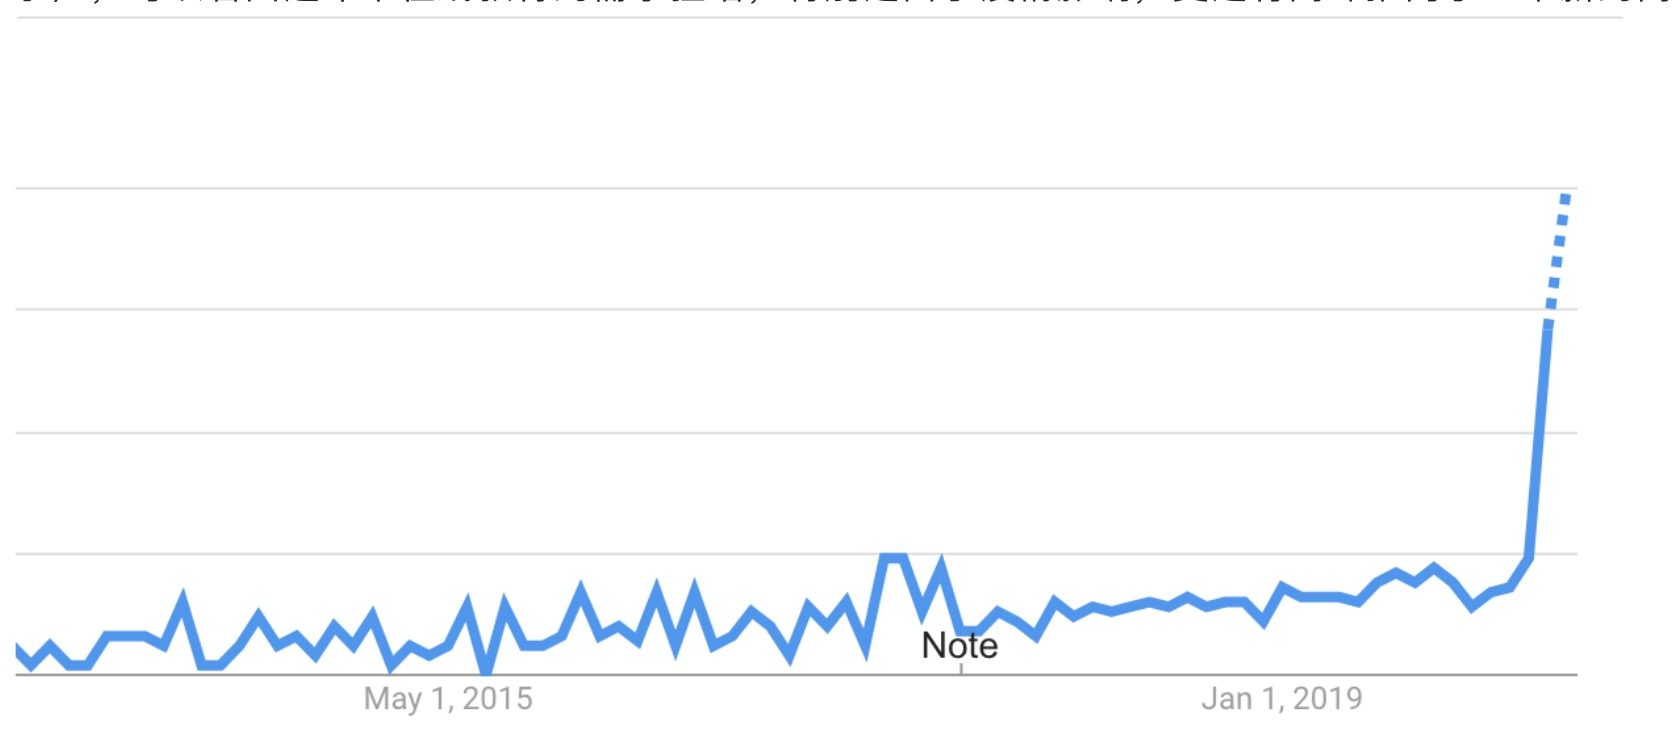
\includegraphics[width=14cm]{网课.png}
\end{center}

另外,随着年轻的开发者不断增多,编程类在线问答网站也越来越受欢迎,根据stackoverflow的用户编程经验统计数据,编程经验少于五年的开发者占了约四成,根据另一张图表:写下第一行代码时候的年龄,可以看出一半的用户在15岁以下就开始学习编程了。

\begin{center}
  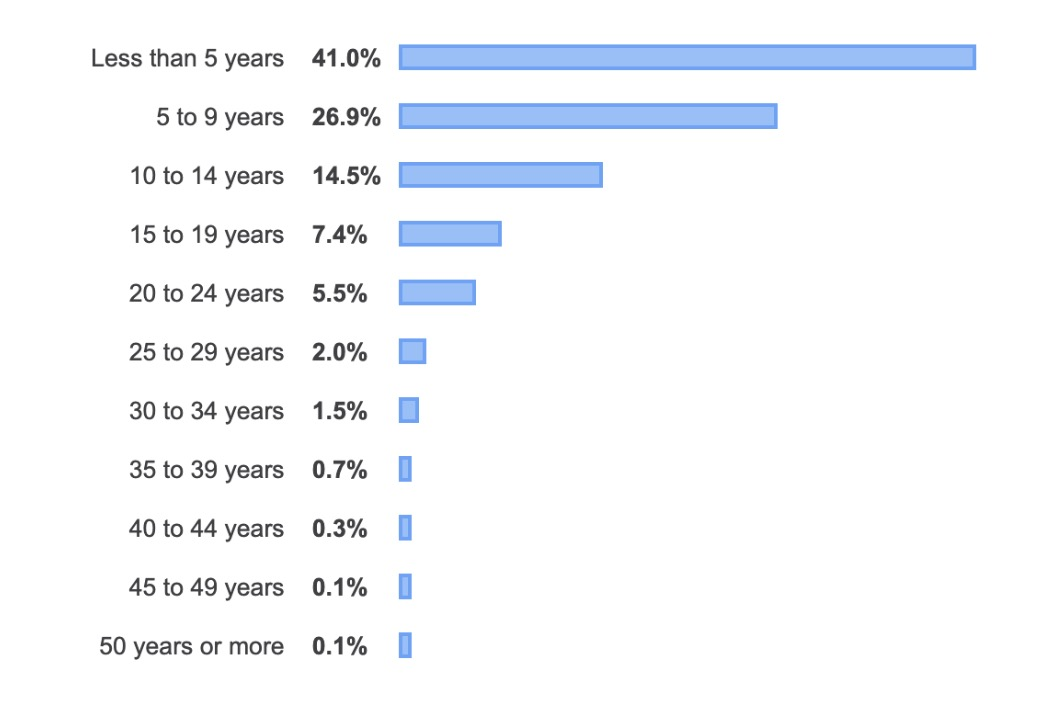
\includegraphics[width=12cm]{第一行代码.png}
\end{center}

对这些年轻的开发者来说,在线教育和问答平台是其学习编程不可或缺的工具,而未来随着计算机相关行业的不断发展,会有更多的、更年轻的开发者加入,因此在线教育和问答平台的市场前景非常广阔,我们平台的价值主张十分契合用户需求。

\begin{center}
  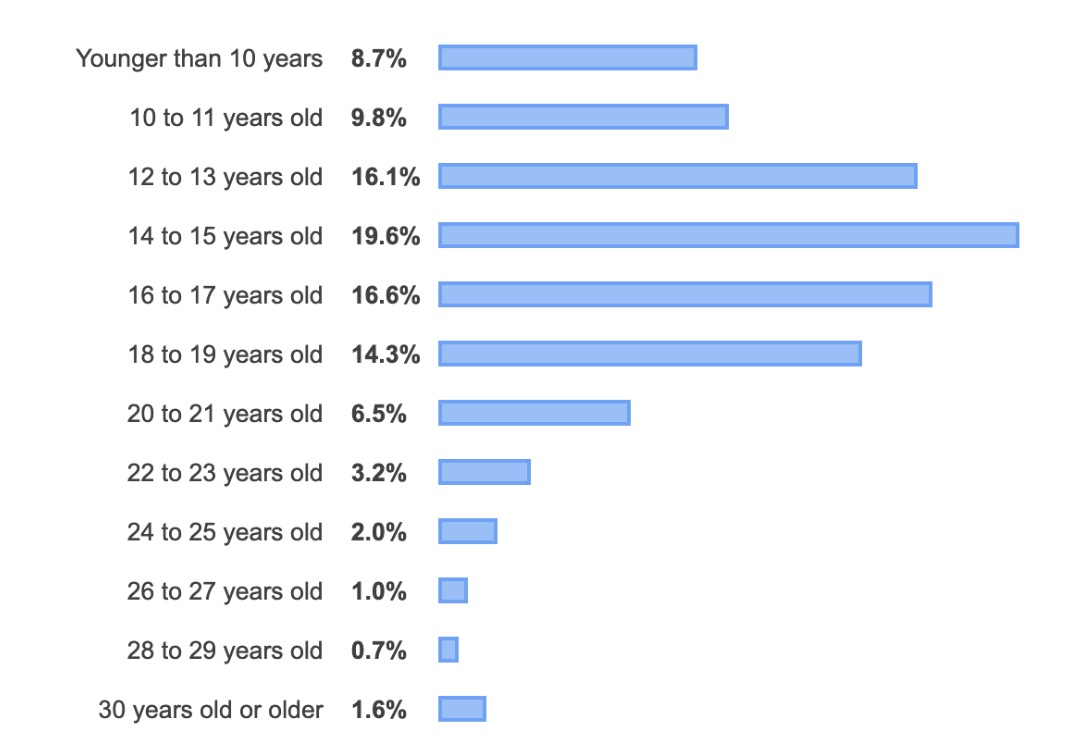
\includegraphics[width=12cm]{年龄.png}
\end{center}

同样,对应着火热的市场,我们的竞争对手也很多,除了stackoverflow之外,还有很多其他的网站集合了问答和文档、社区的功能,市场竞争的激烈是一个潜在的威胁。另外,作为这种用户共同创造的平台,前期需要一定的用户量,因此作为新兴加入竞争的初创公司,我们前期用户量的不足也是我们的劣势所在。

\subsubsection{基础设施评估}
如果能和高校以及企业建立稳固的合作关系,那么我们可以解决前期用户不足导致的课程和回答者的短缺问题。这需要我们加大前期宣传的力度。而在其他的IT基础设施方面,我们可以采用现在流行的云服务来部署我们的业务,因此IT基础设施不是很严重的问题,随着业务规模的扩展,再转为自己购买服务器或开发云服务。

\subsubsection{客户界面评估}
一旦平台形成规模,那么客户的流失率很低,因为一个好用的问答平台和教学网站,一定是有一批优秀的老师和解答者,因此可以持续的解决用户的痛点,用户的粘性高。我们维护客户关系主要是通过社区共同创造和一定程度的私人服务。社区共同创造允许我们贴近用户,了解大部分用户需求,而一对一专属服务可以解决一些特殊用户的问题,这种问题只能由专业的工程师一对一解答。这样我们不仅能把握住用户的普遍需求,也能解决特殊用户的特殊需求,可以维持一个较好的客户关系和渠道。


\section{讲故事}
为了更形象生动地呈现CodeOcean平台的商业模式,我们总共构建了5个故事来帮助理解。其中4个是用户视角故事,第5个是公司视角故事。

\subsection{公司、高校的工程师和老师}
张小林是一位大学副教授,从事软件工程的教学和研究工作已有三十余年,不仅积累了丰富的教学经验,而且对软件工程领域也有相当深入的科研见地,发表了数十篇相关论文。如今已经的他经验丰富,除了在学校任课,他还想帮助更多的人来学习和了解软件工程领域的相关知识。他注意到现在的编程领域的初学者在校内基本还是以学习理论知识为主,对于实践部分还欠缺较多,因此希望在课余时间应用自己丰富的经验给初学者们开设一些偏向实践的课程。他通过调查了解到慕课这样的网课平台,这样的平台对于开设课程的要求都比较高,需要经过层层认证审批,不太适合这种短而精的小课程。而这时,他从其他老师那里了解到学院和CodeOcean平台有深入的合作(\textbf{渠道通路-合作方渠道}),这个平台的网课部分专门设计为开设短而精的课程,只需要简单的教师认证即可开课(\textbf{关键业务-网课教学}),过程简单,十分方便。张教授于是联系和平台的工作人员,很快就通过了认证,可以开设课程了。

在准备课程资料的时候,张教授发现该平台可以根据开课老师的时间来自由安排课程进度(\textbf{价值主张-便捷性}),一点也不会妨碍到自己的本职工作,而且可以有效地利用碎片化时间,这样自己的工作效率得到了巨大的提高。

另外,张老师开设的课程好评如潮,平台还会给张老师一笔不菲的教学费用,作为一项副业,也是一笔可观的收入,张老师在帮助他人之余也获得了物质和精神上的回报,他对此感到十分满意。因此,张老师每周末定期安排和学员的一对一解答服务(\textbf{客户关系-一对一专属私人服务}),这样可以更好地帮助学员答疑解惑。

\subsection{提问者}
Cookie是一个刚刚开始学习编程的大学生。之前对编程一无所知的他,面对大学各种 各样的编程课程感到非常吃力,被一个bug卡住修改到夜里三四点是常有的事;好不容易找了几篇博客来参考,却因为环境不一样常常依赖爆炸;他也尝试询问身边的同学,可是同学们都有各自的作业和任务,没有人有多余时间愿意为 Cookie 耐心讲解。

正当 Cookie 准备自暴自弃,转专业的时候,他无意间(\textbf{渠道通路})听老师同学 提到了CodeOcean平台,巧的是他在学校官网上一下子找到了入口。一进入 CodeOcean,Cookie仿佛发现了新大陆。(\textbf{关键业务})一对一的付费答案外卖保证“解答小哥”随叫随 到,保证准确解决并且理解问题所在;基于docker的问答平台,启用时运用在线版vscode,确保解答者处在提问者一致的环境,而且 展示实时修改结果;与开发 者和社区一同打造的文档(\textbf{重要合作})为用户提供了代码沙盒,妈妈再也不用担心我看不懂文档了。 “(\textbf{价值主张})这也太方便了吧,这样基于答案外卖的问答方式真是让人眼前一亮。”CodeOcean仿佛不 停地在跟Cookie说“用TA,用TA”,Cookie总算找到了一根救命稻草。之前需要花很久才能解决的问题,现在Cookie叫一个答案外卖就可以一键解决了,尽管有时候debug到了深夜,Cookie的答案外卖仍然会有“解答小哥”接单。有时Cookie虽然暂时明白了这个问题,可能过了一两天之后在自己的一番琢磨下又有了一些新的疑惑,他可以通过平台私聊“解答小哥”进行追问。完全解决完问题之后,Cookie通过平台对“解答小哥”支付打赏费用,并且可以为“解答小哥”评星打分。

在CodeOcean的帮助下,Cookie的学习成绩飞速提升,这也吸引了更多的小伙伴加入CodeOcean。

\subsection{编程学员}
陆川是某大学一位名物理学院的学生,出于课程和兴趣,他会时不时地去学习编程,不久前他开始学起了Java语言。但因为本身专业并不是计算机方向,他学起来速度比较慢,有时会以课程多作为借口懈怠了在编程上的学习,以致自己的编程水平在过去一段时间里提升地非常缓慢。考虑到当下慕课之类的在线学习平台数量随着互联网的发展飞速增加,他在想有机会应该去上一两门课程,就像在学校里上课一样。他在网上和与朋友聊天时(\textbf{渠道通路})听说了CodeOcean平台似乎不错,便登上网站想尝试一下,试着参加了一门Java基础学习课程。尝试后感觉还不错,课程本身的进度能监督自己跟上脚步学习,也有老师和同学可以一起讨论,解决他在学习过程中产生的疑问(\textbf{客户关系-教学})。CodeOcean还提供了十分方便的代码沙盒用作教学与讨论工具,基本上只需要自己写代码就行了,不用担心环境配置得不对,比起他以前独自摸索,效率要高多了(\textbf{价值主张-便捷学习})。渐渐地,在CodeOcean上学习成了他日常生活的一环,他希望自己之后能保持在学校之外同时额外学习一门课程(\textbf{知识性资源}),他也很开心地为自己享受的服务支付费用(\textbf{收入来源-课程费用})。他还会考虑向自己身边的想要学习编程的同学推荐这个网站。

\subsection{解答小哥}
林黄是一名软件学院的大学生,每月可以从父母手中获得 2000 元的生活费,虽然不算多,但是也足够他的日常花销了。大二的时候,林黄成功脱单,每月都可以和自己的女朋友约会几次,但是每次约会,少则一百多,多则三四百,林黄的生活费很快就不够用了,但是林黄并不好意思向父母要钱,于是他决定找一份兼职工作。

适逢大三开学,学校正好发布了勤工俭学的通知,林黄毫不犹豫就报了名,他所从事的是图书管理员的工作,每周四下午去学校图书馆工作6小时,一个月可以获得大约450元的工资,这样的收入显然无法满足林黄的需求,只干了一个月,林黄便辞掉了这份工作,就在此时,林黄在网上看到了刷单兼职的广告。广告称只要完成刷单任务,每月可以收入2000元以上,随后,他添加了一位自称刷单工作人员的QQ,并按对方的要求下单了一件10元钱的商品,第二天,林黄果然收到了这笔交易的退款,以及自己的佣金2元。“工作人员”称,为了逃避监管,每人同时只能下一单。之后的几天,他又进行了十几次小额商品的刷单,都获得乐享用的佣金,这彻底消除了林黄的戒备心,随后,“工作人员”告诉林黄,如果下单更加贵的商品,他所能获得的佣金也会成倍增长。林黄仔细考虑后,决定向同学借钱,加上自己的全部生活费,一次性下单了一件5000元的商品,而第二天,林黄却没有如往常一样收到返金,“工作人员”称大额的佣金需要特别审核,将会于3日内发放。可是三天过去了,林黄不但没有收到佣金,反而被“工作人员”拉黑了,惊慌失措的他选择了将此事告诉父母。随后,父母与林黄一同联系了当地警方,但林黄的生活费却无法在短时间内追回。同时,民警也对林黄的刷单行为进行了批评教育,林黄的父母也代替他偿还了向其他同学的钱,这令平时成绩优异、品行优良的他显得异常尴尬。

经过此事,林黄变得十分谨慎,情绪一度十分低落。后来,他无意中发现了CodeOcean这个代码学习平台,在此学习了一段时间后,他对这个平台产生了信任,并决定成为一名“解答小哥”,利用自己的知识来获取解答费。在这个平台上,他可以充分地利用自己掌握的知识,在帮助他人解答问题的同时,自己也学到了新知识。尽管不像刷单平台那样自称月入2000,但是在此收获的解答费也已足够其与女友约会使用。

\subsection{公司视角}
Nyako 是 CodeOcean 平台的CEO,他和他的同事这些年一起度过了无数的不眠之夜才创办出了今天的集网课教学、答案外卖、问答平台、文档中心为一体的开源编程学习平台—— CodeOcean。

Nyako 在上大学期间就注意到了这样的现象,同样是软件工程专业的同学,同学之间能力两极分化严重。有的同学基础比较薄弱,课下需要利用网课学习,甚至有时需要一对一辅导;而有的同学能力很强,甚至可以变成小老师为其他同学解决问题。(\textbf{客户细分})由此 Nyako 发现了商机,创办一个为基础薄弱的同学提供学习上的帮助,还可以为能力强的同学提供良好兼职条件的平台简直是一举两得。基础薄弱的同学可以通过“答案外卖”的方式召唤“解答小哥”解答问题,而能力强的同学通过成为“解答小哥”解答问题收取解答费。而 CodeOcean 公司通过抽取一定比例的解答费用作为收入来源。(\textbf{关键业务-答案外卖}) 

再加上虽然现在各大高校网课资源非常丰富,但是大部分的课程都是面向一学期的,周期很长,而当同学对某一个小的知识点有疑问的时候往往需要的是五分钟左右的短视频来帮助理解。为此 Nyako 联系了许多企业、高校甚至是有影响力的个人开发者,欲和他们合作获得更多的网课资源,然后再将这些资源在平台内部进行审核分类,最后呈现在用户面前(\textbf{重要合作,关键业务,核心资源})。这样一来 CodeOcean 可以对部分优质的网课资源收取课程费用。(\textbf{收入来源})

Nyako 在大学学习期间遇到学业上的困难的时候,有时会上 CSDN,Stack Overflow,这样的问答平台寻找答案。Nyako 认为在这些平台上用户不仅可以使用资源还可以创造资源,同时在无形之中提高了平台的影响力和活跃度(\textbf{关键业务、客户关系})。Nyako 决定将这种问答平台借鉴过来,用户在问答平台上共同创造资源,也可以对某一问题进行深入讨论形成社区。(\textbf{客户关系})

Nyako 回想起自己上大学的时候,看文档总是一件麻烦事儿,干巴巴的代码摆在上面不能自己调试运行显得非常枯燥。Nyako 觉得完全可以将这些代码放在沙盒中直接运行,用户可以随时修改并且观察结果。(\textbf{关键业务})而且和一些开发者、社区合作,收录其开发的项目和文档,并通过 docker 部署一些简单的项目使用代码,可以帮助用户更快上手。这样对于平台和合作方的宣传都有促进作用,从而实现双赢。(\textbf{重要合作})

就这样,初代的 CodeOcean 平台诞生了。但是 Nyako 发现,刚刚诞生的CodeOcean 知名度并不高,很难积累到更多的用户,无法通过自身强渠道来打造良好的口碑。于是他决定利用高校和企业的合作宣传,在企业和高校内举办直播,答疑交流活动。(\textbf{渠道通路})就这样 CodeOcean 的知名度渐渐提升了起来。

渐渐的 CodeOcean 的知名度越来越高,积攒的用户越来越多,但服务器却受不住了。有时候在用户复杂量大的情况下服务器会崩溃,“ CodeOcean 崩了”这样的热搜开始频频出现。“不行,这样会流失用户的。” Nyako 愤愤不平地说,“看来得增加些服务器了。”对于之前小有收益的 CodeOcean 来说,增加一批服务器的费用并不算难事。很快 CodeOcean 进购了一千台高性能的服务器,解决了因为用户量大服务器频频崩溃的问题。(\textbf{核心资源,成本结构})

CodeOcean 平台打着“创新问答,便捷学习”的价值主张(\textbf{价值主张})帮助了越来越多的用户。而此时的CEO Nyako也因为CodeOcean收入不菲,开始赢取白富美,走向人生巅峰。



\section{场景}
虽然使用了故事来帮助商业模式变得更形象化,但故事缺乏背景可能还是会让人感觉抽象和不自然,我们对上述用户视角的故事进行了场景补充,并规范了场景元素使读者能多角度地思考和体会故事的发生场景。(购买与获得要点合并编写)

\subsection{公司、高校的工程师和老师的用户故事场景补充}
\begin{itemize}
  \item \textbf{了解与评估}:张老师是从其他老师那里了解到的,CodeOcean平台和高校有着密切的合作,主要体现在赞助学院的一些晚会活动,邀请老师同学来参观企业,在学院中进行宣传等。通过学院打通和高校的教师的联系。CodeOcean平台的定位和各大主流的网课平台有较大差别,这一点也有利于教师根据自己开设课程的需要来进行评估。
  \item \textbf{购买与传递}:(这里教师和平台不是购买的关系,主要聚焦在传递来讨论)主要还是通过在教师群体中间的传递性,教师这一群体和其他群体的一个区别就是对口碑和熟人营销特别敏感。一般来说如果有一些老师选择某个平台,其他老师也会选择那个平台,因此这里的传递主要还是依赖于教师群体中的口口相传。同时,如果平台有较多的生源,那么对于网络教学来说,教师也会优先考虑有较多观众的平台。
  \item \textbf{交互}:教师群体主要利用平台来开设课程,针对于这一点,平台聚焦于便捷性。CodeOcean和慕课等这些网课平台的一个巨大的不同点就在于“轻量级”,例如中国慕课开设课程会比较正式,需要课程的设计和准备,层层审核,上课的周期和长度也有严格的限制,往往适用于比较正式的网课教学,紧跟课程教学大纲。而CodeOcean平台则从另一个角度,聚焦于“短而精”的课程,这样就给了开课教师极大的灵活性。针对于教师群体来说,时间是一个必须认真思考的问题。教授在学校的本职教学工作和科研工作负担已经很重了,因此我们平台在减轻开课成本上下足了功夫,尽量让教师能轻松开课,聚焦于教学内容的传递而减少不必要的负担。
  \item \textbf{售后}:(主要聚焦于开课后持续的反馈)安排工作人员和老师对接,人工客服7*24小时服务。
  \item \textbf{评价与复购}:主要特现为张老师之后和自己的同事会宣传这个平台,这样会形成用户口碑的良性循环。而后续如果张老师还想开设课程,也会选择我们的平台。
\end{itemize}

\subsection{提问者的用户故事场景补充}
\begin{itemize}
  \item \textbf{了解与评估}:Cookie是从老师同学那儿听说CodeOcean平台的。CodeOcean和一些高校有着密切合作,比如在高校开展技术讲座,VIP促销活动,这促进了老师同学开始了解CodeOcean平台。同时CodeOcean也和一些有名的开发者,社区合作,同学们通过这些有名的开发者社区的广告宣传了解CodeOcean,而且由于是和让人耳熟能详的开发者、社区合作,可以增加信赖度。
  \item \textbf{购买与传递}:Cookie通过打赏”解答小哥“来购买解答服务,购买通过和支付宝,微信这些支付渠道绑定,或者通过扫码付费。对于用户来说非常方便,不需要额外的手续费。提问者大多是在校大学生,学生之间的传递性是非常显著的,一个同学开始使用CodeOcean后,如果觉得为自己提供了不少帮助,会非常乐意分享给舍友或者关系好的同学。
  \item \textbf{交互}:Cookie通过平台发布问题,等待“解答小哥”来解答。平台基于docker,启用时运用在线版vscode,确保解答者处在和Cookie一致的环境,而且展示实时修改结果。而现有的其他平台的提问模块,仅仅是提问者以文字的方式发布问题,解答者不了解提问者的环境,往往无法提供正确的建议。而且CodeOcean尽力扩展“解答小哥”这一用户群体的数量,让提问者的问题在10min之内都能匹配到“解答小哥”解答,保证了解决问题的时效性。
  \item \textbf{售后}:如果Cookie在“解答小哥”的一对一解答之后,仍然存在一些疑问,可以通过平台私聊“解答小哥”,进行追问。并且可以从回答满意度方面为“解答小哥”进行评分。
  \item \textbf{评价与复购}:Cookie之后遇到了问题仍然会优先选择CodeOceanin平台,并且把这个平台安利给了更多的同学。
\end{itemize}

\subsection{编程学员的用户故事场景补充}
\begin{itemize}
  \item \textbf{了解与评估}:在有关慕课的互联网讨论中出现"CodeOcean"的字眼(平台自身渠道,广告等);计算机专业的同学听老师说过后提到(渠道通路的合作方渠道的间接影响)。
  \item \textbf{购买与传递}:陆川找到感兴趣的课程,考虑时间和评价后,为上课资格支付费用。在线学习平台的传递十分简单,买后即可用。
  \item \textbf{交互}:陆川遵循课程时间安排,每周学习最新发布的课程视频(时间不固定),通过代码沙盒提交作业。讨论区中也po出了各个同学的代码沙盒,陆川可以浏览,运行或者尝试修改其代码。
  \item \textbf{售后}:陆川在参加课程的过程中发现课程没有自己想像中的那么有价值,向平台申请,很快地完成了退款流程。
  \item \textbf{评价与复购}:代码沙盒给陆川提供了直观清晰的环境设置与相对统一的代码运行环境,能让他方便地在老师提供的代码沙盒或者同学在讨论区给出的代码沙盒上做实验,能非常快速地吸收和巩固刚学到的知识,免去了配置环境的烦恼。之后他只要时间允许,会选择并为自己感兴趣的课程付费。
\end{itemize}

\subsection{解答小哥的用户故事场景补充}
\begin{itemize}
  \item \textbf{了解与评估}:要提升平台口碑,靠同学之间的相互介绍;与学校合作,经学校向学生进行宣传,增加平台的可信度,吸引更多用户。
  \item \textbf{购买与传递}:无。
  \item \textbf{交互}:解答小哥可以利用自己的空闲时间接单,没有规定的工作时间,更加方便了学生兼职。
  \item \textbf{售后}:平台会对解答小哥的解答过程录像,出现争议时及时介入,保证解答小哥与提问者的权益。
  \item \textbf{评价与复购}:平台对于优质解答次数较多的解答小哥提供额外奖励,增加解答小哥的回答热情,同时也会提高问题的回答效率,吸引到更多用户,达到双赢。
\end{itemize}


\end{document}